%---------------------------------------------------------------------------
%	UNIVERSIDADE FEDERAL DE UBERLÂNDIA
%	Faculdade de Engenharia Elétrica
%	Programa de Pós-Graduação em Engenharia Elétrica
%	Laboratório de Engenharia Biomédica
%	Dissertação de Mestrado
%	Capítulo 3: Metodologia
%---------------------------------------------------------------------------

\section{Materiais e Métodos}

\subsection{Descrição do problema}
O núcleo magnético da figura \ref{circ} é feito de chapas de aço elétrico de grão orientado M-5. O enrolamento é excitado com uma tensão de 60 Hz produzindo no aço uma densidade de fluxo de B = 1.5 sen(\textomega t) [T], onde \textOmega = 2\textpi 60 = 377 rad/s. O aço ocupa 0.94 da área da seção reta. A densidade de massa do aço é 7.65 g/cm3. %Encontre (a) a tensão aplicada, (b) a corrente de pico, (c) a corrente eficaz de excitação e (d) as perdas do núcleo.
\begin{figure}[h]
\centering
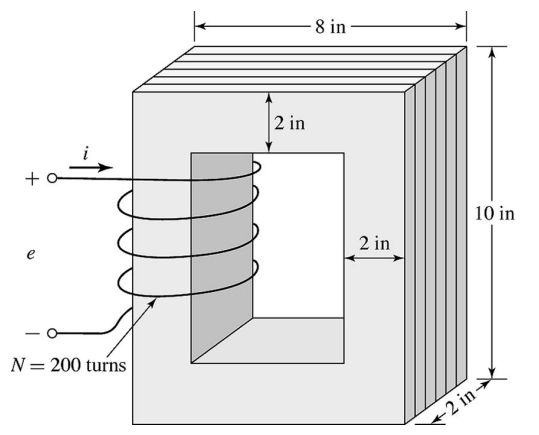
\includegraphics[scale=0.6]{img/assig1/ex1_8.png}
\caption[Núcleo de chapas de aço com um enrolamento]{Núcleo de chapas de aço com um enrolamento. Extraído de \cite{Fitzgerald2008}.}
\label{circ}
\end{figure}

\begin{figure}[H]
\centering
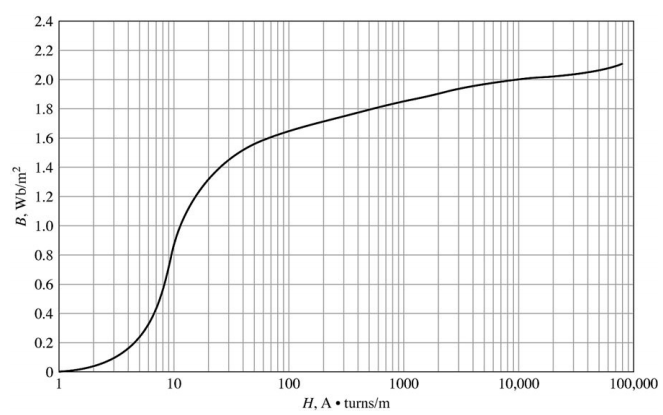
\includegraphics[scale=0.5]{img/assig1/curv_magn.png}
\caption[Curva de magetização CC para o aço elétrico de grão orientado M-5 de 0.012 polegadas de espessura]{Curva de magetização CC para o aço elétrico de grão orientado M-5 de 0.012 polegadas de espessura. Extraído de \cite{Fitzgerald2008}.}
\label{cc}
\end{figure}

\subsection{Ferramenta de elementos finitos: FEMM}
FEMM (Finite Elements Method Magnetics) é um conjunto de programas utilizados para a resolução de problemas eletromagnéticos de baixa frequência em domínios planares (bidimensional) ou assimétricos. O problema permite a resolução dos seguintes tipos de problemas: magnéticos lineares/não-lineares, problemas eletroestáticos lineares, problemas de fluxo de calor e problemas de fluxo de corrente \cite{Meeker2014}.

\subsection{Definições dos parâmetros do problema}
Foram definidos os seguintes parâmetros do problema no FEMM: tipo do problema, unidade de medida, frequência, precisão, ângulo mínimo e método computacional, conforme apresentado na tabela \ref{probdef}.
\begin{table}[H]
\centering
\caption{Parâmetros do problema}
\label{probdef}
\begin{tabular}{ll}
\hline
\textbf{Parâmetro} & \textbf{Descrição} \\ \hline
Tipo do problema   & Planar             \\
Unidade de medida  & Milimetros         \\
Frequência (Hz)    & 0                  \\
Precisão           & 1E-008             \\
Ângulo Mín         & 30º                \\
Método             & Aprox. Suc         \\ \hline
\end{tabular}
\end{table}

\subsection{Cálculo da área do condutor}
\begin{equation}
Area_{condutor} = \frac{i}{D_{cu}} = \frac{0.1 [A]}{2.5 [\frac{A}{mm^2}]} = 0.04 [mm^2]
\end{equation}

Achando o valor de diâmetro:
\begin{equation}
Area_{condutor} = \frac{\pi d^2}{4}
\end{equation}
\begin{equation}
d = \sqrt[]{\frac{4 \times Area_{condutor}}{\pi}} = 0.225676 [mm]
\end{equation}

Como não há disponível um material com o valor de diâmetro igual a 0.225676 [mm], adota-se o material com medida mais próxima. O material escolhido foi o 30AWG, com diâmetro igual a 0.254724 [mm]. A partir do novo diâmetro, realiza-se o cálculo para Área'.

\begin{equation}
Area_{condutor}' = \frac{\pi d^2}{4} = \frac{\pi 0.254724^2}{4} = 0.050960 [mm^2]
\end{equation}

Conforme a descrição do problema o enrolamento possui 200 espiras. Dessa forma:
\begin{equation}
AreaT_{condutor}' = N_{espiras} * Area_{condutor}' = 200 * 0.050960 [mm^2]
\end{equation}
\begin{equation}
AreaT_{condutor}' =  10.192026 [mm^2] \approx 10 [mm^2]
\end{equation}

A partir do valor da área total do condutor, considerando as 200 espiras, é possível encontrar diversas medidas que possuam o valor de área de 10 [mm\textsuperscript{2}]:
\begin{itemize}
\item 10.0 [mm] X 1.0 [mm]
\item  5.0 [mm] X 2.0 [mm]
\item  4.0 [mm] X 2.5 [mm]
\end{itemize}
Para a construção da espira no circuito magnético, optou-se pelas dimensões 5.0 X 2.0 [mm].

\subsection{Construção do circuito magnético no FEMM}
O problema foi reconstruido na camada de interação. A camada de interação do FEMM possui uma barra de ferramentas (Figura \ref{ferramentas}) que permite a construção de objetos geométricos bidimensionais. A partir dai são inseridos os pontos e os segmentos de retas para construção do circuito magnético análogo do enunciado do problema.
\begin{figure}[H]
\centering
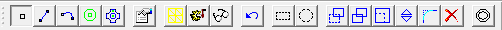
\includegraphics[scale=1]{img/assig1/ferram.png}
\caption[Barra de ferramentas]{Barra de ferramentas.}
\label{ferramentas}
\end{figure}

\begin{figure}[H]
\centering
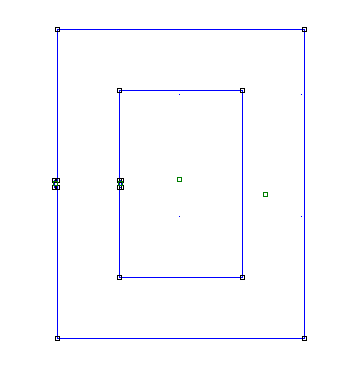
\includegraphics[scale=0.65]{img/assig1/circ_mag1.png}
\caption[Circuito magnético no FEMM]{Circuito magnético no FEMM}
\label{circ_mag}
\end{figure}

\subsection{Definição dos materiais a serem utilizados}
Após a construção geométrica do circuito magnético, é necessário atribuir os materiais a serem utilizados. O FEMM disponibiliza uma biblioteca de materiais com parâmetros definidos.
\begin{table}[H]
\centering
\caption{Materiais}
\label{mat}
\begin{tabular}{lll}
\hline
\textbf{Material} & \textbf{sigma {[}MS/m{]}} & \textbf{Atributos especiais} \\ \hline
Ar                & 0                         & Não laminado                 \\
US Steel Type 2-S & 6.25                      & Laminado no plano            \\
30 AWG            & 58                        & Fio magnético                \\ \hline
\end{tabular}
\end{table}


\subsection{Definição dos circuitos}
Foram definidos dois circuitos para o problema:
\begin{itemize}
\item Icurr (Corrente do circuito série com 0.1 [A])
\item -Icurr (Corrente do circuito série com -0.1 [A])
\end{itemize}

\begin{figure}[H]
\centering
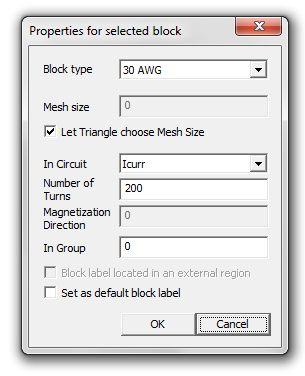
\includegraphics[scale=1]{img/assig1/circ_1.png}
\caption[Propriedades para o circuito Icurr]{Propriedades para o circuito Icurr}
\label{icurr_p}
\end{figure}

\begin{figure}[H]
\centering
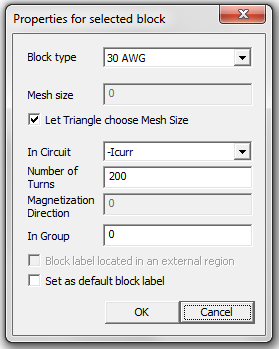
\includegraphics[scale=1]{img/assig1/circ_2.png}
\caption[Propriedades para o circuito -Icurr]{Propriedades para o circuito -Icurr}
\label{icurr_m}
\end{figure}

\subsection{Condições de contorno}
As condições de contorno delimitam as dimensões do problema. A partir das condições de contorno foram definidas as regiões do problema (ar, enrolamento eo circuito magnético). Uma vez definidas as regiões, foram atribuidos os materiais específicos de cada uma delas.

\begin{figure}[H]
\centering
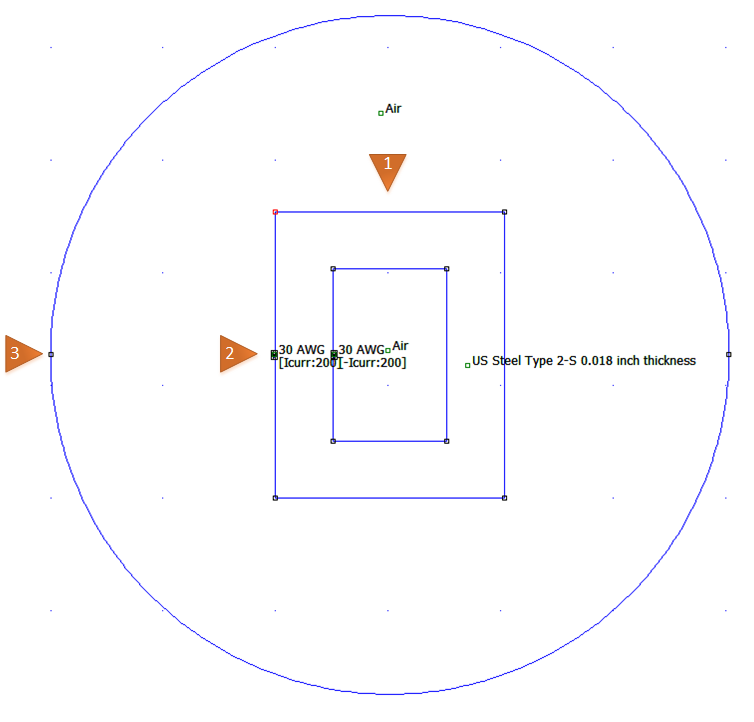
\includegraphics[scale=0.65]{img/assig1/circ_mag.png}
\caption[Circuito magnético, enrolamento, fronteira]{1) Circuito Magnético; 2) enrolamento; 3) fronteira circular}
\label{circ_mag}
\end{figure}
